\documentclass[11pt,a4paper]{article}
\usepackage[utf8]{vietnam}
\usepackage[margin=2cm]{geometry}
\usepackage{graphicx}
\usepackage{xcolor}
\usepackage{tcolorbox}
\usepackage{hyperref}
\usepackage{booktabs}
\usepackage{tabularx}
\usepackage{enumitem}
\usepackage{tikz}
\usetikzlibrary{shapes,arrows,positioning,calc}

% Theme Colors
\definecolor{navybg}{HTML}{060C1A}
\definecolor{goldprimary}{HTML}{E0C588}
\definecolor{golddark}{HTML}{C5A059}
\definecolor{cardbg}{HTML}{091326}
\definecolor{accentgreen}{HTML}{10B981}
\definecolor{accentred}{HTML}{EF4444}
\definecolor{accentblue}{HTML}{3B82F6}

\hypersetup{
    colorlinks=true,
    linkcolor=golddark,
    filecolor=golddark,      
    urlcolor=golddark,
    pdftitle={Cam Nang Van Hanh OlymQuiz Arena},
    pdfpagemode=FullScreen,
}

\tcbuselibrary{skins,breakable}

\newtcolorbox{stepbox}[1]{
    colback=cardbg,
    colframe=goldprimary,
    fonttitle=\bfseries\color{navybg},
    coltitle=navybg,
    colbacktitle=goldprimary,
    enhanced,
    attach boxed title to top left={yshift=-2mm,xshift=4mm},
    boxed title style={sharp corners,rounded corners=northwest,rounded corners=northeast},
    title=#1,
    boxrule=1pt,
    arc=3mm,
    top=4mm,bottom=3mm,left=3mm,right=3mm
}

\newtcolorbox{tipbox}[1]{
    colback=cardbg,
    colframe=accentgreen,
    fonttitle=\bfseries\color{white},
    coltitle=white,
    colbacktitle=accentgreen,
    enhanced,
    title=#1,
    boxrule=1pt,
    arc=2mm,
    top=2mm,bottom=2mm,left=3mm,right=3mm
}

\begin{document}

% --- TITLE PAGE ---
\begin{titlepage}
    \pagecolor{navybg}
    \color{white}
    \begin{center}
        \vspace*{1.5cm}
        
        
\begin{tikzpicture}
            \draw[goldprimary, fill=goldprimary!20, line width=2pt] (0,0) circle (1.2cm);
            \node at (0,0) {\color{goldprimary}\Huge\bfseries $\Omega$};
        \end{tikzpicture}
        
        \vspace{0.8cm}
        {\Huge\bfseries\color{goldprimary} OLYMQUIZ ARENA}\\[0.3cm]
        {\large\bfseries\color{slate!80} HỆ THỐNG ĐẤU TRƯỜNG ĐỐI KHÁNG TRỰC TIẾP 4 BỤC}\\[1.5cm]
        
        \begin{tcolorbox}[colback=cardbg,colframe=goldprimary!50,arc=4mm,width=0.85\textwidth,halign=center]
            \color{white}
            \vspace{0.2cm}
            {\Large\bfseries CẨM NANG VẬN HÀNH BỎ TÚI}\\[0.2cm]
            {\normalsize Dành cho Ban Giám Khảo, Điều Hành \& Thí Sinh}\\[0.2cm]
            \color{goldprimary}\small\textit{Ngắn gọn -- Trực quan -- Dễ hiểu trong 1 nốt nhạc}
            \vspace{0.2cm}
        \end{tcolorbox}
        
        \vfill
        
        {\small Website: \url{https://olymquiz.vercel.app}}\\[0.2cm]
        {\footnotesize Phiên bản Nobel Academic -- Bản quyền © 2026 OlymQuiz Arena}
        
        \vspace{1cm}
    \end{center}
\end{titlepage}

\nopagecolor
\color{black}

% --- PHẦN 1: QUY TRÌNH 3 BƯỚC VẬN HÀNH NHANH ---
\section*{\color{navybg}⚡ QUY TRÌNH 3 BƯỚC ĐIỀU HÀNH TRẬN ĐẤU}
Chỉ cần nắm vững 3 bước này là có thể vận hành trọn vẹn một trận thi đấu:

\begin{stepbox}{BƯỚC 1: CẤP MÃ PIN CHO 4 THÍ SINH}
\begin{enumerate}[leftmargin=*]
    \item Ban Giám Khảo mở trang \textbf{Quản lý 4 thí sinh} (\url{/admin/players}).
    \item Bấm nút \textbf{[Sao chép Link thi đấu]} của từng máy (Máy 1, 2, 3, 4) gửi cho 4 bạn thí sinh kèm mã PIN (Ví dụ: \texttt{1111}, \texttt{2222}, \texttt{3333}, \texttt{4444}).
    \item Thí sinh mở link trên điện thoại/laptop và nhập mã PIN để vào bục đấu.
\end{enumerate}
\end{stepbox}

\begin{stepbox}{BƯỚC 2: BẮT ĐẦU CÂU HỎI \& CHẤM ĐIỂM (DÙNG PHÍM TẮT)}
\begin{enumerate}[leftmargin=*]
    \item Chọn câu hỏi $\rightarrow$ Nhấn phím \textbf{[Space]} để bắt đầu đếm ngược thời gian.
    \item Hết giờ: Hệ thống tự động khóa nộp bài (hoặc bấm phím \textbf{[L]} để khóa chủ động).
    \item Bấm \textbf{[Mở Đáp Án]} để chiếu đáp án lên màn hình máy chiếu.
    \item Nhấn phím \textbf{[G]} để \textbf{Chấm điểm tự động} (Điểm sẽ được cộng ngay lập tức vào bảng tổng).
\end{enumerate}
\end{stepbox}

\begin{stepbox}{BƯỚC 3: CHIẾU SLIDE VINH DANH \& TRAO GIẢI}
\begin{enumerate}[leftmargin=*]
    \item Khi kết thúc 4 vòng thi, Ban Giám Khảo bấm nút \textbf{[4. Bảng Vàng Trao Giải]}.
    \item Màn hình máy chiếu lập tức phát hiệu ứng Pháo hoa Confetti và vinh danh Quán quân cùng thứ hạng 4 thí sinh.
\end{enumerate}
\end{stepbox}

\vspace{0.5cm}

% --- PHẦN 2: BÀN ĐIỀU HÀNH BAN GIÁM KHẢO ---
\section*{\color{navybg}🎛️ CHI TIẾT CÁC NÚT TẠI BÀN GIÁM KHẢO (/admin/live)}

\begin{figure}[h!]
    \centering
    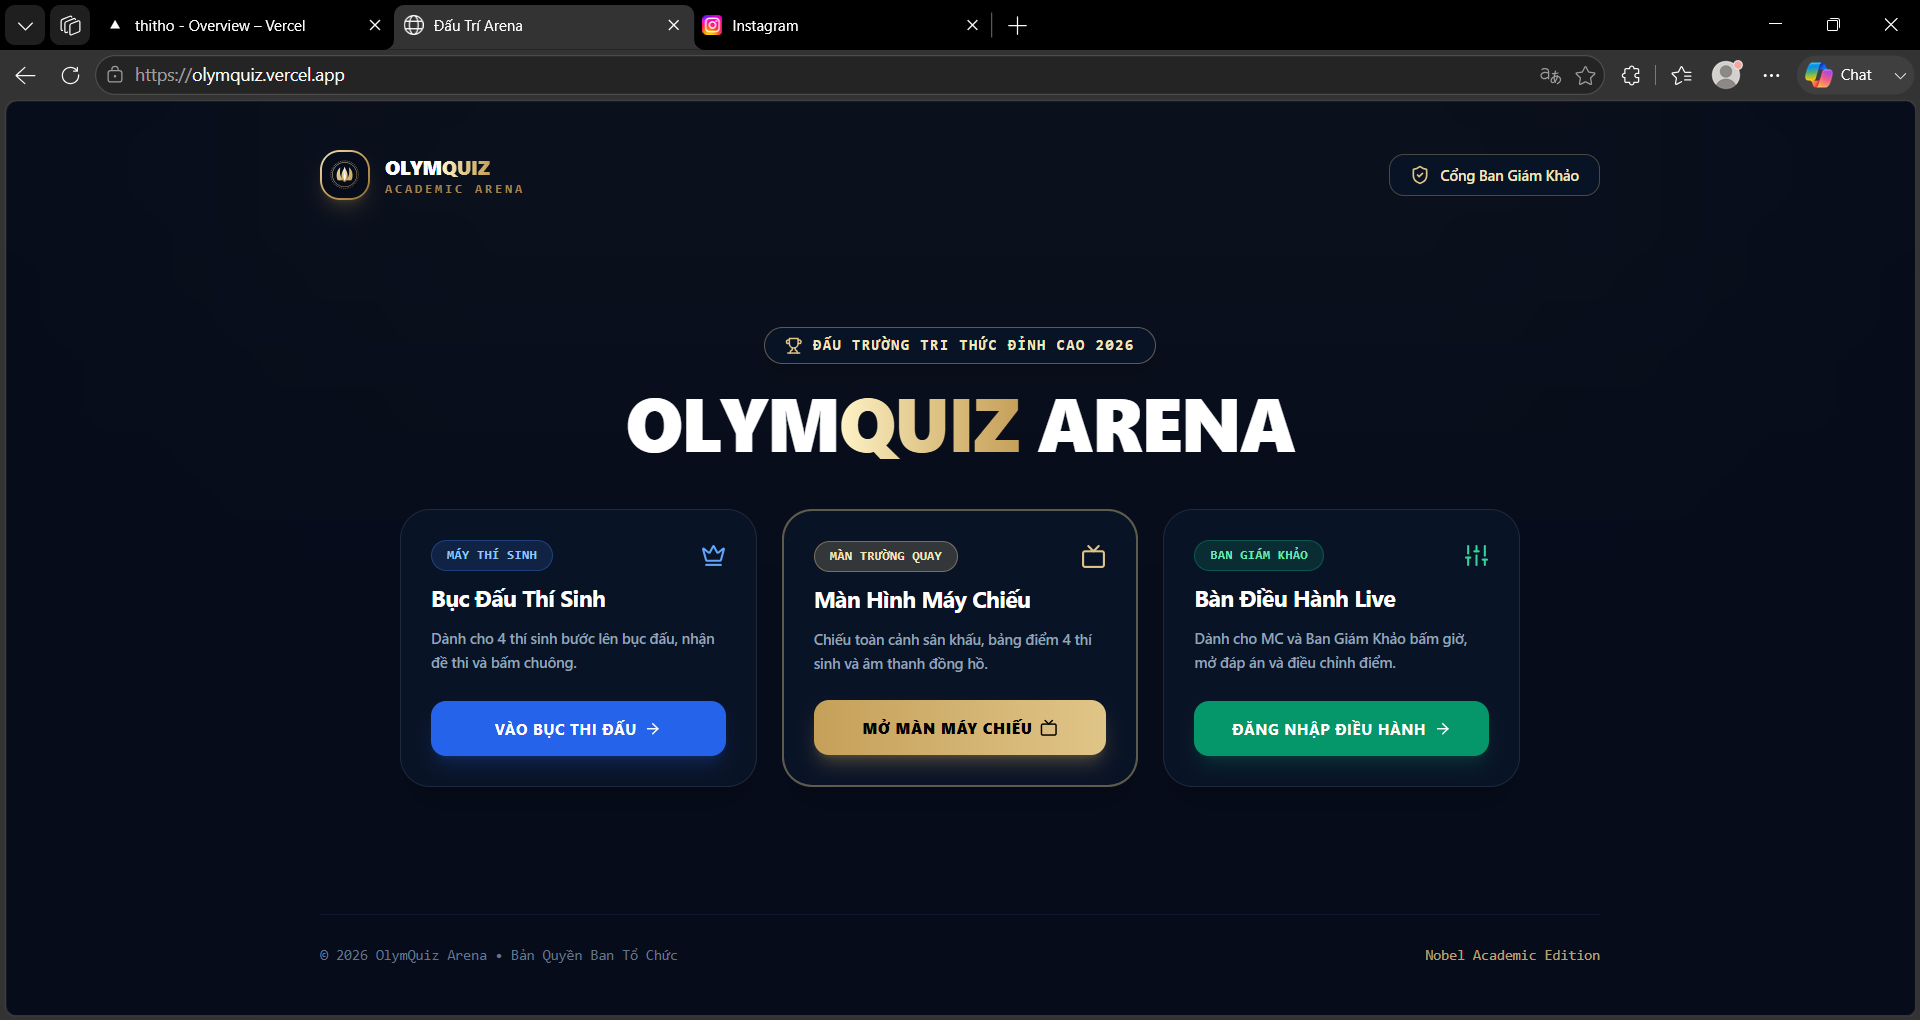
\includegraphics[width=0.95\textwidth]{screenshots/13_admin_live.png}
    \caption{Giao diện Bàn Giám Khảo Live với các cụm điều khiển trực quan}
\end{figure}

\begin{table}[h!]
\centering
\small
\begin{tabularx}{\textwidth}{l p{3.5cm} X}
\toprule
\textbf{Ký hiệu} & \textbf{Tên nút chức năng} & \textbf{Ý nghĩa \& Hành động} \\
\midrule
\textbf{[1] Timer} & \textbf{Bắt Đầu / Tạm Dừng} & Phím \texttt{Space}: Chạy hoặc dừng đồng hồ đếm ngược. \\
\textbf{[2] Reset} & \textbf{Reset (R)} & Phím \texttt{R}: Trả đồng hồ về mặc định \& xóa bài nộp tạm thời. \\
\textbf{[3] Khóa} & \textbf{Khóa Nộp (L)} & Phím \texttt{L}: Khóa/Mở quyền bấm chọn của 4 thí sinh. \\
\textbf{[4] Mở} & \textbf{Mở Đáp Án} & Chiếu đáp án đúng lên máy chiếu và bục thí sinh. \\
\textbf{[5] Chấm} & \textbf{Chấm Điểm (G)} & Phím \texttt{G}: Tự động kiểm tra đúng/sai và cộng điểm. \\
\textbf{[6] Slides} & \textbf{Thanh Chọn Slide} & Chuyển đổi giữa 5 chế độ: Câu hỏi, Giới thiệu, Luật thi, Bảng vàng, Standby. \\
\textbf{[7] Sao} & \textbf{Sao Hy Vọng} & Bật/Tắt cờ Ngôi Sao Hy Vọng ở Vòng 4 (+x2 hoặc -50\%). \\
\textbf{[8] Chuông} & \textbf{Reset Chuông} & Mở lại chuông cướp điểm khi thí sinh trước trả lời xong. \\
\textbf{[9] Điểm} & \textbf{+20 / +30 / -10} & Bộ nút cộng/trừ điểm thủ công nhanh cho từng thí sinh. \\
\bottomrule
\end{tabularx}
\end{table}

\vspace{0.3cm}

% --- PHẦN 3: BỤC THÍ SINH ---
\newpage
\section*{\color{navybg}📱 GIAO DIỆN BỤC THÍ SINH (/player/1 -- /player/4)}

\begin{figure}[h!]
    \centering
    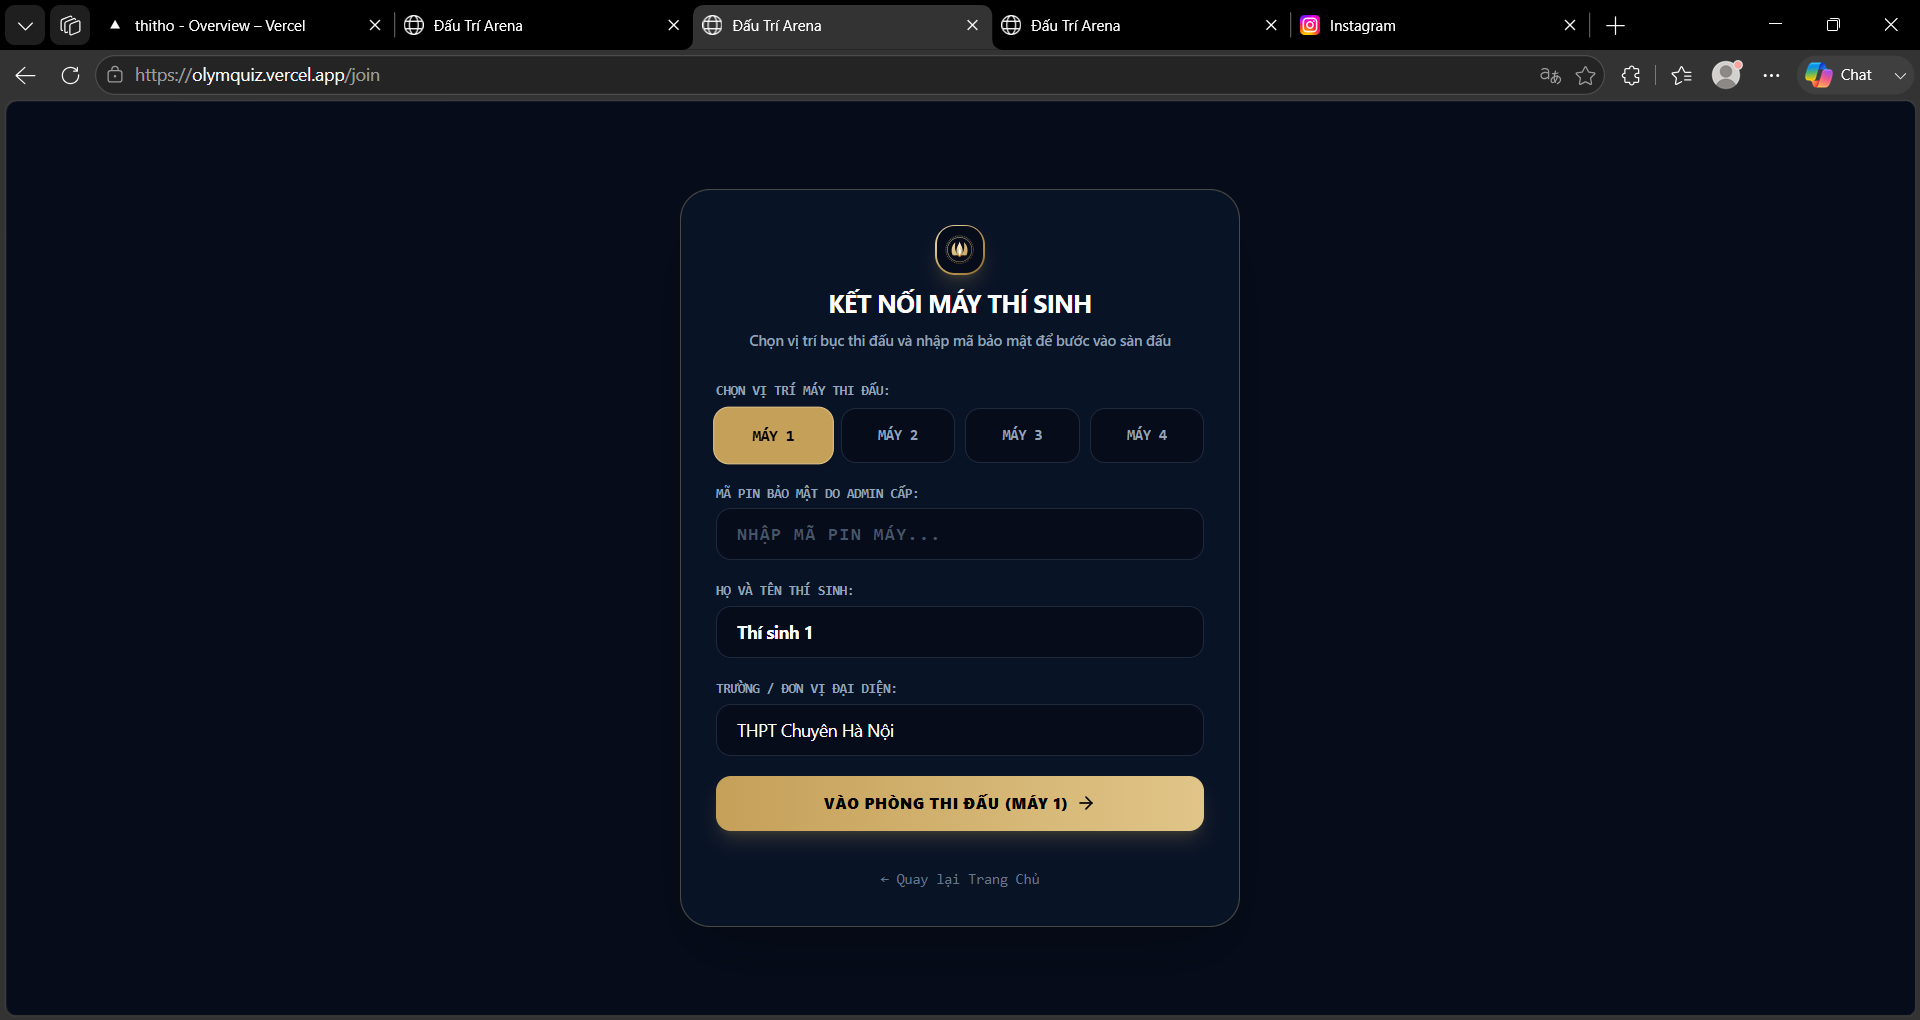
\includegraphics[width=0.85\textwidth]{screenshots/11_player_screen.png}
    \caption{Giao diện Bục Thí Sinh với 4 nút trắc nghiệm lớn Touch Cards}
\end{figure}

\begin{stepbox}{CÁCH THÍ SINH THAO TÁC TRÊN MÁY:}
\begin{itemize}[leftmargin=*]
    \item \textbf{1. Trắc nghiệm (Vòng 1 \& 3)}: Chạm trực tiếp vào ô \textbf{A, B, C, D}. Nút sẽ sáng đèn xác nhận nộp bài thành công kèm thời gian nộp (mili-giây).
    \item \textbf{2. Tự luận / Ô chữ (Vòng 2)}: Gõ chữ vào ô nhập và bấm nút \textbf{[Nộp Bài]}.
    \item \textbf{3. Cướp điểm (Vòng 4)}: Nút chuông đỏ to \textbf{[BẤM CHUÔNG GIÀNH QUYỀN]} sẽ sáng lên, ai bấm nhanh nhất sẽ giành được quyền trả lời.
    \item \textbf{4. Đặt Sao Hy Vọng}: Nhấn nút \textbf{[⭐ ĐẶT NGÔI SAO HY VỌNG]} trước khi bắt đầu câu hỏi của mình ở Vòng Về Đích.
\end{itemize}
\end{stepbox}

\vspace{0.5cm}

% --- PHẦN 4: 5 CHẾ ĐỘ SLIDE MÁY CHIẾU ---
\section*{\color{navybg}🖥️ 5 CHẾ ĐỘ SLIDE TRÌNH CHIẾU MÁY CHIẾU (/display)}

Ban Giám Khảo có thể chuyển đổi linh hoạt 5 chế độ Slide bất kỳ lúc nào:

\begin{table}[h!]
\centering
\small
\begin{tabularx}{\textwidth}{l l X}
\toprule
\textbf{Chế độ Slide} & \textbf{Tên Slide} & \textbf{Mục đích sử dụng} \\
\midrule
\textbf{Slide 1} & \textbf{Câu Hỏi Thi Đấu} & Chiếu đề bài, 4 phương án, Laser Timer và 4 bục điểm. \\
\textbf{Slide 2} & \textbf{Giới Thiệu 4 Thí Sinh} & Chiếu toàn cảnh hồ sơ 4 bạn bước lên sân khấu. \\
\textbf{Slide 3} & \textbf{Toàn Bộ 4 Vòng} & Chiếu bảng thể lệ tổng quan 4 vòng đấu cho hội trường. \\
\textbf{Slide 3.1--3.4} & \textbf{Luật Vòng 1/2/3/4} & Chiếu chi tiết thể lệ riêng của từng vòng trước khi bắt đầu. \\
\textbf{Slide 4} & \textbf{Bảng Vàng Trao Giải} & Bục vinh danh Quán quân + Pháo hoa chúc mừng chung cuộc. \\
\textbf{Slide 5} & \textbf{Màn Hình Chờ Standby} & Chiếu Logo Nguyệt Quế 4K khi nghỉ giải lao hoặc chuẩn bị. \\
\bottomrule
\end{tabularx}
\end{table}

\begin{figure}[h!]
    \centering
    \begin{minipage}{0.48\textwidth}
        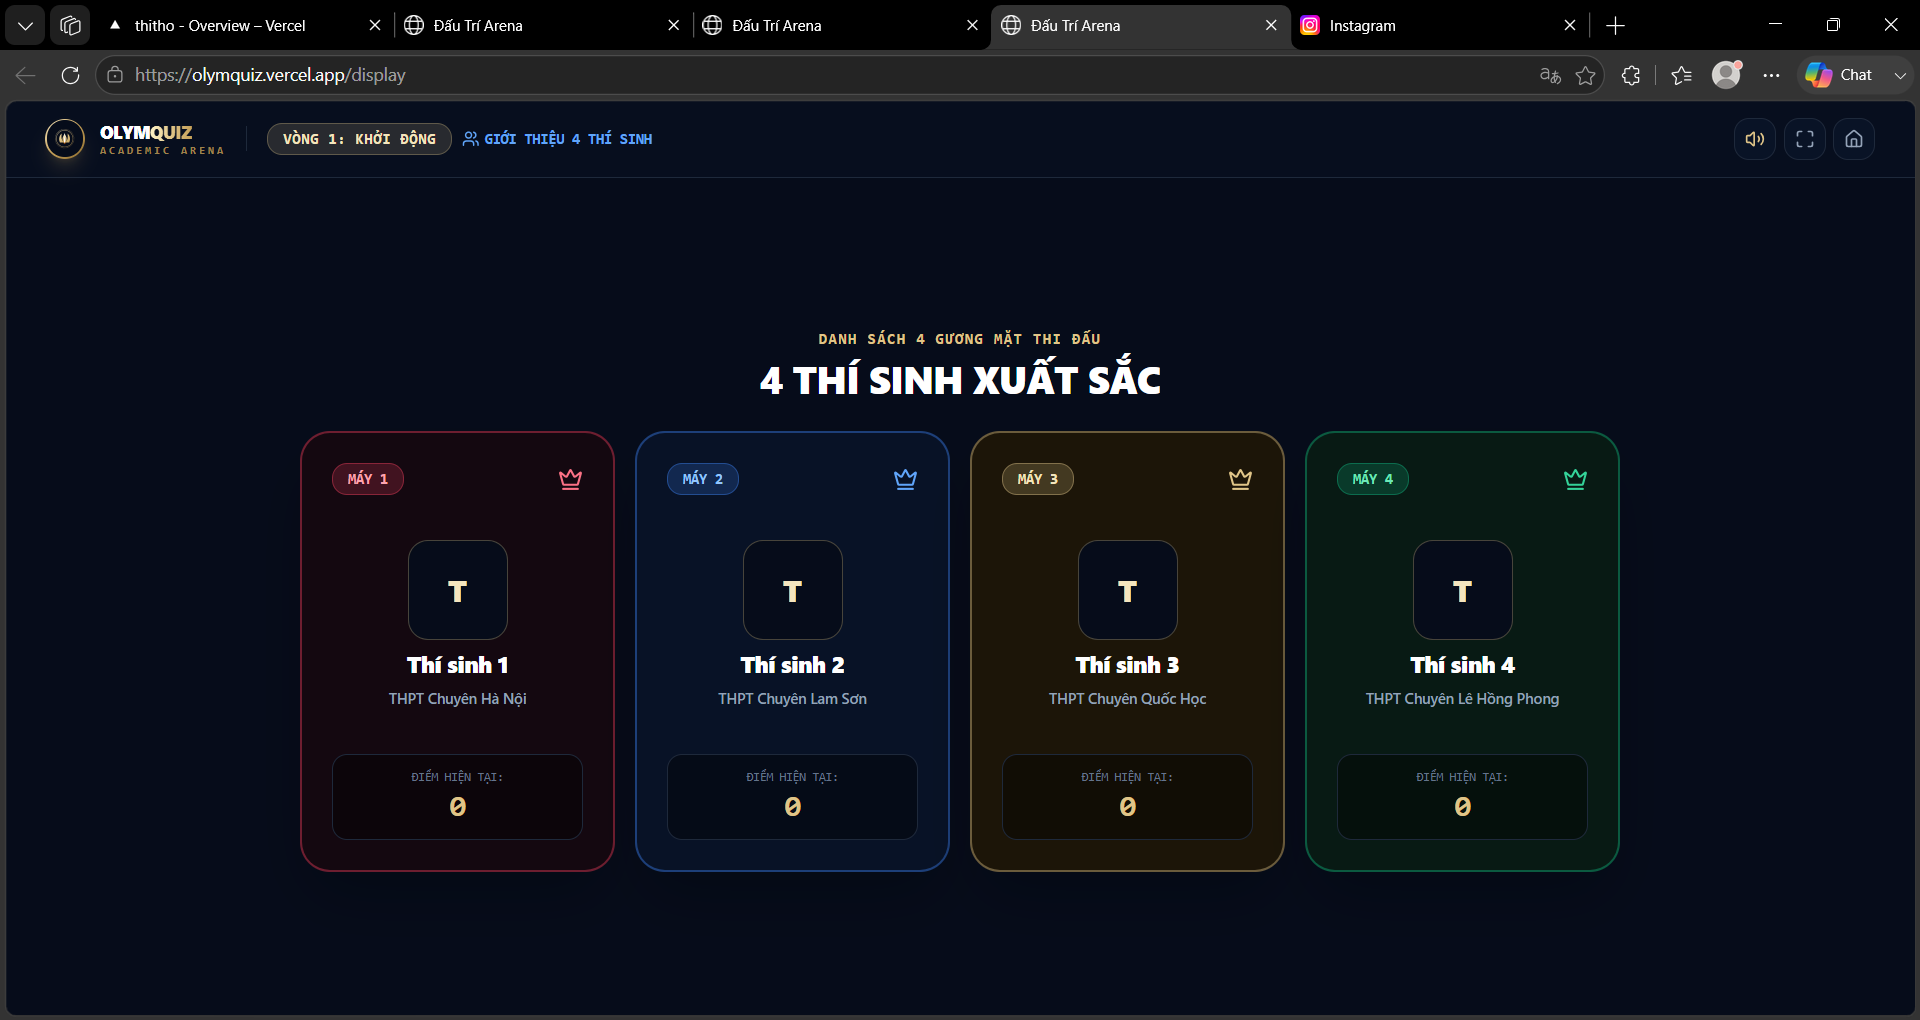
\includegraphics[width=\textwidth]{screenshots/04_display_intro.png}
        \caption{Slide Giới thiệu 4 Thí Sinh}
    \end{minipage}
    \hfill
    \begin{minipage}{0.48\textwidth}
        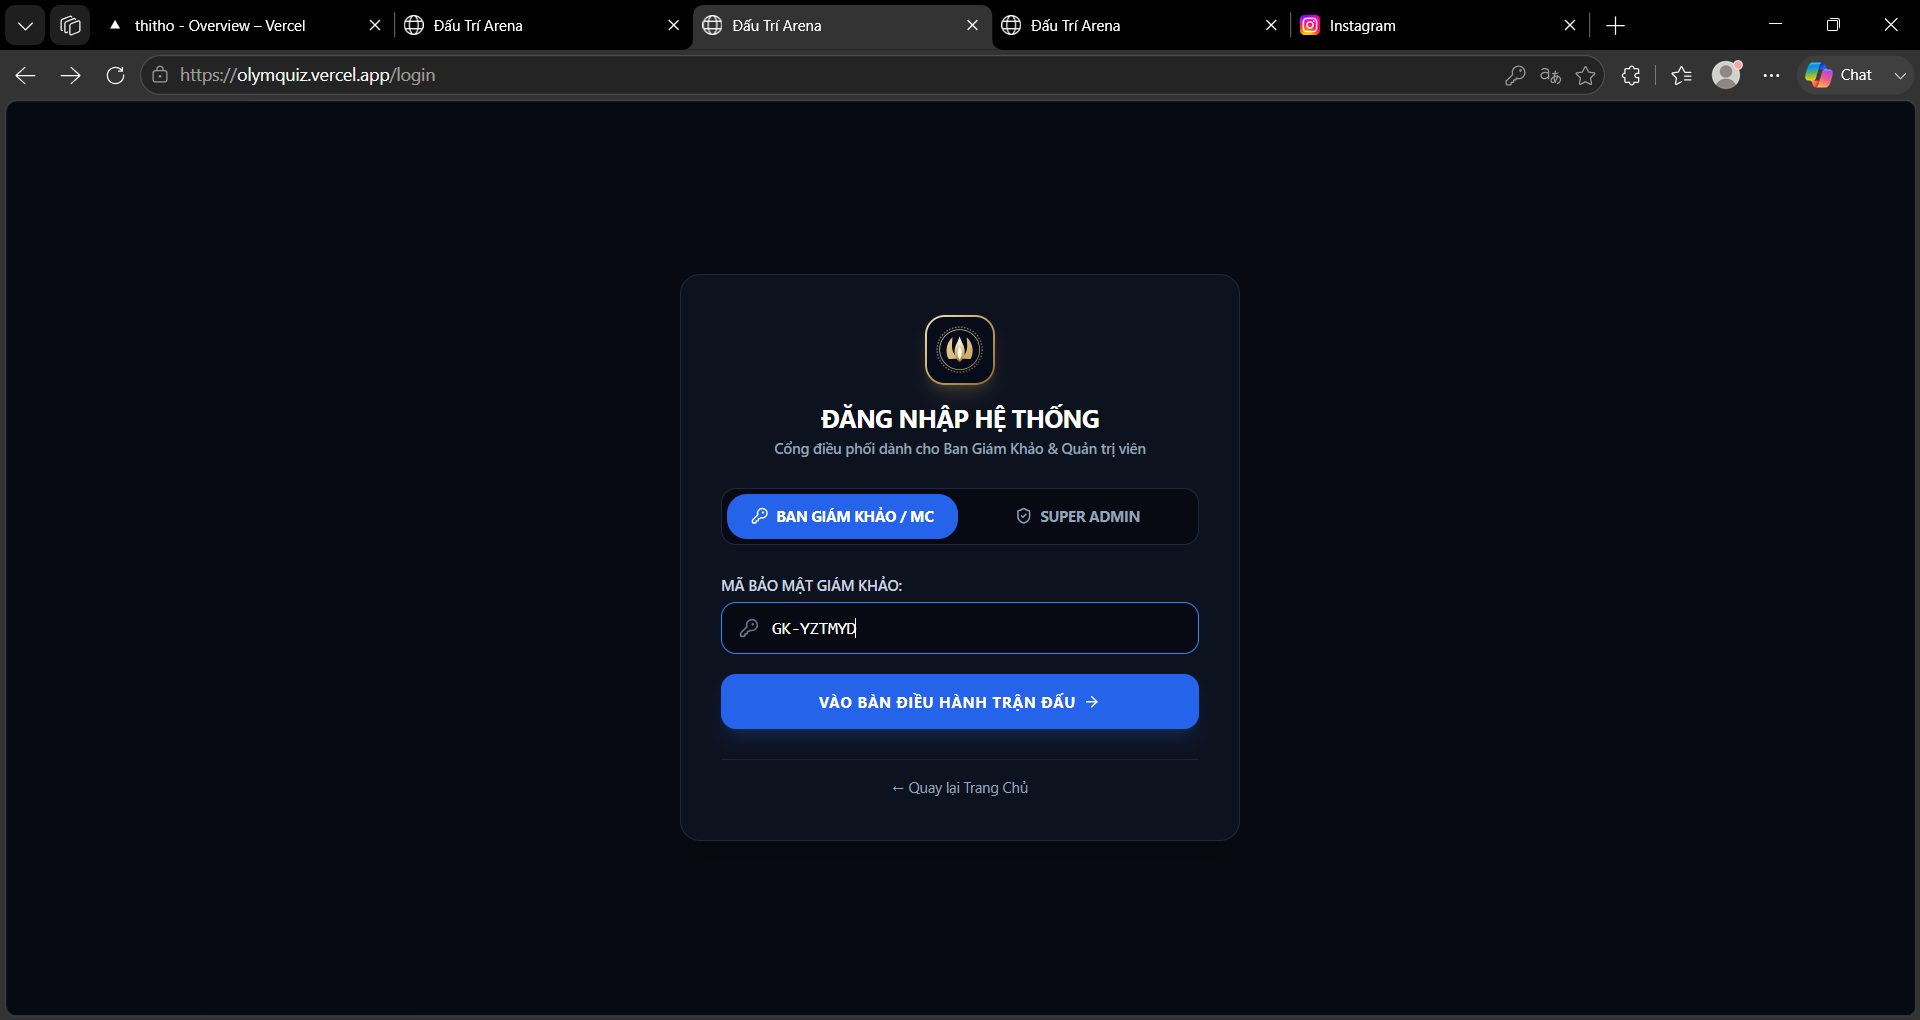
\includegraphics[width=\textwidth]{screenshots/10_display_leaderboard.png}
        \caption{Slide Bảng Vàng Trao Giải}
    \end{minipage}
\end{figure}

\vspace{0.3cm}

\begin{tipbox}{MẸO VẬN HÀNH THUẬN TIỆN CHO GIÁM KHẢO}
\begin{itemize}[leftmargin=*]
    \item Hãy bấm phím \textbf{F11} trên màn hình máy chiếu \url{/display} để vào chế độ Fullscreen toàn màn hình đẹp nhất.
    \item Dùng 3 phím tắt vàng: \textbf{Space} (Đếm giờ) $\rightarrow$ \textbf{L} (Khóa bài) $\rightarrow$ \textbf{G} (Chấm điểm) giúp trận đấu diễn ra mượt mà và chuyên nghiệp như truyền hình trực tiếp!
\end{itemize}
\end{tipbox}

\end{document}
